\chapter{Алгоритмы и методы решения}
\label{chap:solution}

\section{Получение исходных текстов}

Прежде чем индексировать данные, необходимо научиться их автоматически получать и помещать в хранилище для дальнейшего доступа.

Предполагается, что в качестве системы контроля версий используется Git. Поэтому предлагаемое решение использует особенности его работы, чтобы более эффективно сохранять данные.

Git хранит всё содержимое репозитория с использованием двух видов объектов: \textbf{деревья} (trees) и файлы (blobs). Каждое дерево представляет собой директорию и хранит в себе список своих непосредственных потомков: всех поддеревьев и всех файлов. Каждый объект является неизменяемым и имеет уникальный идентификатор. В случае, если содержимое файла не изменилось, то его идентификатор не меняется и переиспользуется объект из предыдущего состояния репозитория. В случае же, если в файле были некоторые изменения, то создается новый объект файла и содержащее его \textbf{дерево} клонируется таким образом, чтобы указывать на новую версию файла (и старые версии неизменившихся файлов). Аналогично изменения распространяются до самого корня репозитория. Всё это позволяет указывать на любую версию репозитория с помощью единственного идентификатора корневого \textbf{дерева}, и при этом переиспользовать неизменившиеся между версиями объекты.

Чтение данных напрямую из репозитория, однако, довольно затруднено. С одной стороны, Git не позволяет эффективных способов доступа к отдельным объектам без выкачивания всего репозитория (потому что объекты, бывает, группируются и сжимаются вместе). С другой стороны, доступ к серверу часто ограничен авторизацией и большая читающая нагрузка может создать на него неожиданную нагрузку. Для обхода этих ограничений, предлагаемый Сервис хранит копию всех данных из Git-репозитория в собственной базе данных.

Процесс синхронизации изменений выглядит следующим образом:

\begin{enumerate}
    \item При помощи команды \texttt{git pull} на диск выкачивается актуальное состояние репозитория;
    \item Чтением объектов из директории \texttt{.git} определяется текущее корневое дерево и собирается список всех файлов и всех директории в текущем состоянии репозитория. При этом пропускаются все директории и файлы, которые уже были обработаны ранее.
    \item Найденные объекты загружаются в базу данных.
\end{enumerate}

Это позволяет эффективно находить все изменения в репозитории и не дублировать файлы в хранилище Сервиса.

К сожалению, Git не позволяет общего метода узнавать об изменениях, кроме как периодически проверяя их наличие. Сервис предоставляет все механизмы для индексации того или иного репозитория, но его запуск возлагается на пользователя — это может быть настроенный на создание новых коммитов webhook на стороне сервиса вроде Gitlab или Bitbucket, или может быть cron-задача, индексирующая репозиторий время от времени.

\section{Получение семантических данных}

Исходя из сформулированных требований, помимо получения текстового содержимого репозитория, также необходимо получить семантическую информацию о коде: информация о символах в коде и связях между ними.

Учитывая необходимость индексировать различные проекты на различных языках программирования, нужно использовать универсальный и расширяемый метод для индексации. Существует несколько разных подходящих механизмов получения необходимой информации:

\begin{itemize}
    \item Google Kythe \cite{Kythe} — одна из первых попыток предоставить независящий от языка API для получения информации о коде. Несмотря на богатые возможности, проект не пользуется популярностью вне Google, а количество поддерживаемых языков весьма ограничено.
    \item Language Server Index Format (LSIF) \cite{lsif} — формат, построенный вокруг экосистемы Language Server. Имеет детальную документацию и поддерживается большим количеством языков программирования (за счет отдельных анализаторов исходного кода для каждого языка).
    \item SCIP Code Intelligence Protocol (SCIP) \cite{scip} — развитие LSIF для применения внутри Sourcegraph. Более эффективен, чем LSIF, но сложнее в интеграции и использовании.
\end{itemize}

Исходя из простоты использования и наиболее широкой поддержкой сообществом, для реализации был выбран \gls{LSIF}.

Модель \gls{LSIF} представляет собой граф, в котором описываются различные виды узлов и описываются связи между ними. Ключевым для данного проекта является вид узлов, соответствующим подстрокам в исходном коде индексируемого проекта. Так, например, для следующего кода будет, среди прочих, найдено два узла, представляющие собой подстроки «foo» и «self».
\begin{minted}{Python}
def foo(self):
    pass
\end{minted}

Каждая подстрока задается номером строки, началом и длиной, а также может иметь тег. Затем эти для этих подстрок в графе формируются ребра, описывающие результаты вызова метода Language Server (например, \texttt{textDocument/definition}) по отношению к этим подстрокам, а также их принадлежность к тем или иным файлам.

При обработке графа, выполняется две задачи. Во-первых, все подстроки привязываются к ранее загруженному в базу данных файлу из Git-репозитория. Во-вторых, в базу данных копируются все ребра и узлы графа. Причем важно понимать, что результат индексирования одного файла могут меняться при изменении совершенно других. Эта особенность требует также реализовать механизмы версионирования и для всех объектов, описывающие граф. Более подробно модель данных описывается в разделе \fullref{section:data-model}.

\section{Пользовательский интерфейс}

Пользовательский интерфейс реализован с помощью специальной сборки Visual Studio Code, которая работает прямо в браузере пользователя. Встроенное в неё расширение обеспечивает взаимодействие с бекендом: отображение всех файлов, предоставление подсказок, функциональность навигации.

Расширение решает три задачи:
\begin{enumerate}
    \item Предоставляет реализацию виртуальной файловой системы, доступной только на чтение и загружающее файлы и деревья с сервера.
    \item Указывает для VSCode способ взаимодействия с реализацией \gls{LSP}, работающей на бекенде.
    \item Предоставляет команды для выбора текущей версии репозитория.
\end{enumerate}

Бекенд, в свою очередь представляет API для доступа к:

\begin{enumerate}
    \item Списку версий репозитория (со ссылкой на корневую директорию этой версии);
    \item Доступ к объектам файлов и объектам директорий;
    \item API для выполнения LSP-запросов, с указанием используемой версии репозитория.
\end{enumerate}

Все запросы к API осуществляются с помощью HTTP. Более подробно оно описывается в разделе \fullref{section:api}.

\section{Алгоритм формирования ответа на запрос LSP-клиента}
\label{lsp-algorithm}

Среди всех видов вершин графа \gls{LSIF} можно выделить наиболее важные:
\begin{itemize}
    \item \texttt{Range} — вершины, указывающие на некоторую подстроку в файле;
    \item \texttt{[…]Result} — вершины, хранящие результат того или иного запроса;
    \item \texttt{ResultSet} — вершины, агрегирующие результаты для нескольких похожих подстрок. Например, для одной и той же функции «get» во всех местах будет отображаться одна и та же информация при наведении курсора, независимо от конкретного места использования функции.
\end{itemize}

Также рассмотрим некоторые виды рёбер:

\begin{itemize}
    \item \texttt{Next} — соединяет вершину \texttt{Range} и все связанные с ней вершины \texttt{ResultSet}.
    \item \texttt{Item} — для каждой вершины-результата связывает с ней подстроки, которые входят в ответ.
    \item \texttt{Definition}, \texttt{Hover}, \texttt{References} и т.п. — соответствуют методам запросов в протоколе \gls{LSP} и связывают \texttt{ResultSet} с соответствующими результатами запросов.
\end{itemize}

\begin{figure}[H]
    \centering
    \includesvg[inkscapelatex=false, width=\textwidth, height=0.5\textheight]{figures/lsif.svg}
    \caption{Изображение подграфа, содержащего информацию о функции «get».}
    \label{fig:lsif-graph}
\end{figure}

Алгоритм ответа на запрос «найти определение \glslink{symbol}{символа}, расположенного в файле $D$ под $N$-ым символом на строке $L$, используя версию репозитория $V$» будет состоять из следующих операций:

\begin{enumerate}
    \item Найти в базе данных объект файла $D$.
    \item Найти в нём строку $L$.
    \item Найти в базе данных все проиндексированные подстроки, которые содержатся внутри найденной строки $L$ и одновременно в версии $V$.
    \item Среди них выбрать те подстроки, которые включают в себя $N$-ый символ (на рисунке соответствующая подстроке вершина графа выделена цветом).
    \item Для данных подстрок, используя ребра \texttt{Next}, найти все связанные с ними узлы типа \texttt{ResultSet}.
    \item Найти в графе рёбра с типом \texttt{Definition}, связывающие найденные \texttt{ResultSet} и узел, содержащий результат запроса. Ожидается найти только единственный такой.
    \item \label{item-definitions} Найти в графе ребро с типом \texttt{Item}, соединенное с результатом запроса. Другими словами, найти все узлы графа, которые входят в данный результат.
    \item Это ребро будет соединять результат запроса с подстрокой, соответствующей искомому определению.
    \item Для подстроки можно найти файл, в котором та находится, а затем, с использованием всей этой информации, сформировать ответ пользователю.
\end{enumerate}

Аналогичным образом можно находить все использования символа (в п. \ref{item-definitions} алгоритма необходимо выбирать ребра со свойством «References»), а также отвечать на любые другие запросы, необходимые в рамках данного проекта.

\section{Версионирование данных}

Поскольку сервис допускает просмотр различных версий репозитория, остро встает вопрос об эффективном хранении всех необходимых данных. Если же данные Git-репозитория возможно представить в виде дерева, в котором различные поддеревья могут быть переиспользованы в различных версиях, то хранение семантического графа невозможно представить таким образом, поскольку тот не имеет единого естественного корня, не является ориентированным, да и необходимость создавать новую версию каждого предка при изменении единственного узла приводит к очень большому количеству новых объектов в достаточно плотно связанном графе. Поэтому для семантических данных необходимо использовать другой подход к версионированию.

Для этого возьмём за основу подход Multiversion Concurrency Control (MVCC) \cite{reed78mvcc} и для каждого объекта (например, узел или ребро графа) будем указывать две версии: когда этот объект был создан и когда этот объект был удален (если был). Это позволит легко находить только те объекты, которые действительно существуют в любой заданной версии, просто проверяю текущую версию на предмет вхождения в интервал для каждого проверяемого объекта.

\begin{figure}[H]
    \centering
    \begin{tikzpicture}[scale=\textwidth/8.3cm]
        \begin{scope}[shift={(0, -0.3)}]
            \node[circle, draw, minimum size=0.3cm] (x1) at (0, 0) {$x$};
            \node[above=0cm of x1] (x1l) {\scriptsize $[1…]$};

            \node[circle, draw, minimum size=0.3cm] (y1) at (1.5, 0.3) {$y$};
            \node[above=0cm of y1] (y1l) {\scriptsize $[1…2]$};
            
            \draw (x1) -- (y1) node [midway, above, sloped] {\scriptsize $[1…2]$};
        \end{scope}
        \node[draw,dotted,fit=(x1)(x1l)(y1)(y1l), label=below:{версия $1$}] (g1) {};
        
        \begin{scope}[shift={(3,0)}]
            \node[circle, draw, minimum size=0.3cm] (x2) at (0, 0) {$x$};
            \node[above=0cm of x2] (x2l) {\scriptsize $[1…]$};

            \node[circle, draw, minimum size=0.3cm] (y2) at (1.5, 0.3) {$y$};
            \node[above=0cm of y2] (y2l) {\scriptsize $[1…2]$};
            
            \node[circle, draw, minimum size=0.3cm] (z2) at (1.5, -0.3) {$z$};
            \node[below=0cm of z2] (z2l) {\scriptsize $[2…]$};
            
            \draw (x2) -- (y2) node [midway, above, sloped] {\scriptsize $[1…2]$};
            \draw (x2) -- (z2) node [midway, below, sloped] {\scriptsize $[2…]$};
        \end{scope}
        \node[draw,dotted,fit=(x2)(x2l)(y2)(y2l)(z2)(z2l), label=below:{версия $2$}] (g2) {};
        
        \begin{scope}[shift={(6,0.15)}]
            \node[circle, draw, minimum size=0.3cm] (x3) at (0, 0) {$x$};
            \node[above=0cm of x3] (x3l) {\scriptsize $[1…]$};
            
            \node[circle, draw, minimum size=0.3cm] (z3) at (1.5, -0.3) {$z$};
            \node[below=0cm of z3] (z3l) {\scriptsize $[2…]$};
            
            \draw (x3) -- (z3) node [midway, below, sloped] {\scriptsize $[2…]$};
        \end{scope}
        \node[draw,dotted,fit=(x3)(x3l)(z3)(z3l), label=below:{версия $3$}] (g3) {};
        
        \draw [->,decoration={snake,amplitude=.4mm,segment length=2mm,post length=1mm},shorten >=1pt,shorten <=1pt]
            (g1) edge[decorate] (g2)
            (g2) edge[decorate] (g3);
    \end{tikzpicture}
    \caption{пример создания новых версий графа}
\end{figure}

Однако это потребует ввести отношение порядка на версиях репозитория, что не всегда возможно, поскольку в Git-репозиториях существуют и активно применяются ветки.

\begin{figure}[H]
    \centering
    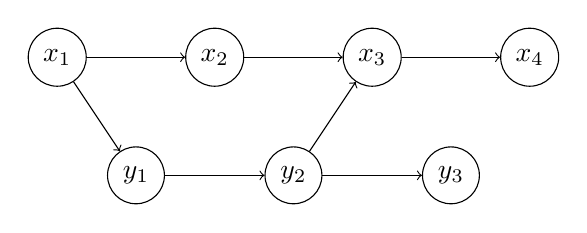
\begin{tikzpicture}
        \node[circle, draw] (x1) at (0, 0) {$x_1$};
        \node[circle, draw] (x2) at (2, 0) {$x_2$};
        \node[circle, draw] (x3) at (4, 0) {$x_3$};
        \node[circle, draw] (x4) at (6, 0) {$x_4$};
        
        \node[circle, draw] (y1) at (1, -1.5) {$y_1$};
        \node[circle, draw] (y2) at (3, -1.5) {$y_2$};
        \node[circle, draw] (y3) at (5, -1.5) {$y_3$};
        
        \draw[->]
            (x1) edge (x2)
            (x2) edge (x3)
            (x3) edge (x4)
            (y1) edge (y2)
            (y2) edge (y3)
            (x1) edge (y1)
            (y2) edge (x3);
    \end{tikzpicture}
    \caption{возможные связи коммитов в репозитории с несколькими ветками}
    \label{fig:multicommits}
\end{figure}

В связи с этим нельзя ответить на вопрос «находится ли коммит $x$ после коммита $y$» — в некоторых случаях они могут быть несравнимы (например, $x_4$ и $y_4$ на рис. \ref{fig:multicommits}).

Чтобы разрешить эту проблему, разделим граф Git-коммитов на набор непрерывных отрезков таким образом, чтобы можно было ввести отношение порядка между всеми коммитами в рамках одного отрезка. Обычно каждый коммит входит в тот же отрезок, в котором находится его родитель, кроме двух следующих случаев. Во-первых, будем начинать новый отрезок когда родительский коммит уже имеет по меньшей мере одного ребенка (например, $y_1$ начинает новый отрезок). Во-вторых, всегда будем начинать новый отрезок, если коммит имеет более одного родителя (как, например, $x_3$). Каждому отрезку дадим уникальный идентификатор, а каждому коммиту внутри него — порядковый номер.

\begin{figure}[H]
    \centering
    \begin{tikzpicture}
        \node[circle, draw] (x1) at (0, 0) {$x_1$};
        \node[circle, draw] (x2) at (2, 0) {$x_2$};
        \node[circle, draw] (x3) at (4, 0) {$x_3$};
        \node[circle, draw] (x4) at (6, 0) {$x_4$};
        
        \node[circle, draw] (y1) at (1, -1.5) {$y_1$};
        \node[circle, draw] (y2) at (3, -1.5) {$y_2$};
        \node[circle, draw] (y3) at (5, -1.5) {$y_3$};
        
        \draw[->]
            (x1) edge (x2)
            (x2) edge (x3)
            (x3) edge (x4)
            (y1) edge (y2)
            (y2) edge (y3)
            (x1) edge (y1)
            (y2) edge (x3);
        
        \begin{scope}[on background layer]
            \node[draw,fill=yellow,dotted,fit=(x1) (x2), label={отрезок $\alpha$}] {};
            \node[draw,fill=yellow,dotted,fit=(y1) (y2) (y3), label=below:{отрезок $\beta$}] {};
            \node[draw,fill=yellow,dotted,fit=(x3) (x4), label={отрезок $\gamma$}] {};
        \end{scope}
    \end{tikzpicture}
    \caption{выделенные непрерывные отрезки}
\end{figure}

Также начнем для каждого версионируемого объекта будем хранить набор промежутков, в которые тот существует — по одному промежутку для каждого известного нам отрезка. Каждый промежуток указывает, в какой коммит объект был создан (если был создан) и в какой был удален (если был удален). Если объект не был ни создан, ни удален в отдельно взятом отрезке, то можно не сохранять в объект промежуток, соответствующий данному отрезку. Это позволит легко вводить новые отрезки без необходимости обновлять все ранее существовавшие объекты.

Тогда, при необходимости проверить, принадлежит ли некоторый объект версии репозитория $(n, m)$ (где $n$ — идентификатор отрезка, а $m$ — порядковый номер коммита в нём), можно воспользоваться следующим алгоритмом:
\begin{enumerate}
    \item Если объект содержит промежуток для отрезка $n$, то достаточно будет лишь проверить, что число $m$ входит в этот промежуток.
    \item В противном случае, мы знаем, что объект не был ни удален, ни создан в отрезке $n$. Тогда нужно рассмотреть коммиты $p_1, …, p_k$, которые являются родителями самого первого коммита рассматриваемого отрезка. Если объект существует хотя бы в одном из них, то это будет означать, что он существовал до начала отрезка $n$ и при этом не был в нём удален, а следовательно объект существует. Аналогично из отсутствия объекта во всех родителях следует и его отсутствие в текущей версии.
\end{enumerate}

В последнем шаге можно избавиться от рекурсии, если заранее собрать для каждого отрезка упорядоченный набор отрезков-родителей всех уровней, обойдя в ширину дерево наследования отрезков. При этом необходимо сперва проверять наличие объекта в тех отрезках, которые находятся «ближе» по дереву наследования.

\section{Спекулятивная индексация}

Поскольку индексация текста с помощью \gls{LSIF} может занимать продолжительное время, имеет смысл для более новых версий Git-репозитория отдавать индексы, построенные на более ранних.

Для этого заметим, что большая часть коммитов не влияет значительно на семантическую информацию, которая связана с неизменившимися частями кода. Поэтому мы можем для неизменившихся строк отдавать ответы, основываясь на информации, полученной из одной из предыдущих версий репозитория.

Во-первых, необходимо представить каждый файл из Git-репозитория как упорядоченный набор строк. Каждая строка будет иметь уникальный идентификатор, к которому будут привязываться результаты индексации с помощью \gls{LSIF} (вместо привязки к номеру строки в файле). Это позволит при добавлении новых строк в середину файла продолжить использовать ранее построенные индексы.

Во-вторых, при запросе подсказки на конкретной строке, если для запрашиваемой версии индексы ещё не были построены, то необходимо найти ближайшую версию, на которой индексы для этой строки строились. Затем остается отдать индексы, связанные с этой строкой, используя найденную версию.

Эти индексы могут быть не вполне корректными (например, при поиске использований символа, если в версии было добавлено новое использование, ещё не проиндексированное). Но в большом количестве случаев они окажутся достаточно полезными, поскольку часто в коммите меняется лишь сравнительно небольшая часть кода и ценно предоставить пользователю индексы для неизменившихся частей, которые часто даже будут верными.

\section{Выводы по главе}

В этой главе были описаны алгоритмы и методы, лежащие в основе разрабатываемой системы. Они позволяют создать реализацию, эффективно решающую поставленные задачи. Получение данных напрямую из Git-репозитория позволяет использовать некоторые особенности системы контроля версий для ускорения загрузки данных и избежать хранения дублирующих объектов. Метод получения семантических данных о коде позволяет легко добавлять поддержку новых языков и переиспользует уже существующие решения данной задачи. Выбранный подход к реализации пользовательского интерфейса, с одной стороны, прост в интеграции с системой и имеющимися семантическими данными, а с другой — предоставляет хорошо знакомый многим разработчикам интерфейс, что облегчает использование системы. Также приводится подробный алгоритм, позволяющий вычислять необходимые ответы на запросы пользователя с использованием ранее полученных данных. Наконец, в этой главе описывается метод версионирования данных в хранилище. обеспечивающий, с одной стороны, возможность использования данных из предыдущих версий репозитория, а с другой — позволяющий эффективно сохранять результаты индексации в базе данных без излишнего дублирования.

\clearpage